\documentclass[12pt]{article}
\usepackage{titling}
\usepackage{graphicx}
\usepackage[top=1in, bottom=1.5in, left=1in, right=1in]{geometry}

%\setlength{\droptitle}{-10em}

\title{Designing an Embedded Microcontroller Laboratory}
\author{Team 12 \\ Stuart Larsen \ \ \ \ \   Troy Drabek \\ Keegan Larkin \ \ \ \ \   Adam Funkenbusch }
\date{\today}

\begin{document}
\maketitle
\thispagestyle{empty}

\pagebreak
\begin{abstract}

  This document gives a brief overview of the designs for the embedded microcontroller laboratory. \\

  \noindent
  The current design for the laboratory entails multiple lab benches configured to ease in the development of software systems for popular microcontroller and embedded systems. Included in the laboratory will also be a station for the fabrication of new custom embedded systems.

\end{abstract}

\thispagestyle{empty}
\pagebreak

\tableofcontents
\thispagestyle{empty}
\pagebreak
\setcounter{page}{1}


\section{Overview}

\section{Team Members}
\begin{center}
  \begin{tabular}{  l | p{8cm} | l }
    Name & Position & Email \\
    \hline
    Stuart Larsen & Project Lead & sclarsen@mtu.edu \\ 
    Troy Drabek & Expert in Microcontroller Design & tqdrabek@mtu.edu \\
    Keegan Larkin & Expert in Fabrication and Synthsis of Macro Quantum Electrodynamic Embedded Devices  & kjlarkin@mtu.edu \\
    Adam Funkenbusch & Expert wire cutter & aefunken@mtu.edu \\

  \end{tabular}
\end{center}

\section{Embedded Devices}

\subsection{MSP430}
\begin{center}
  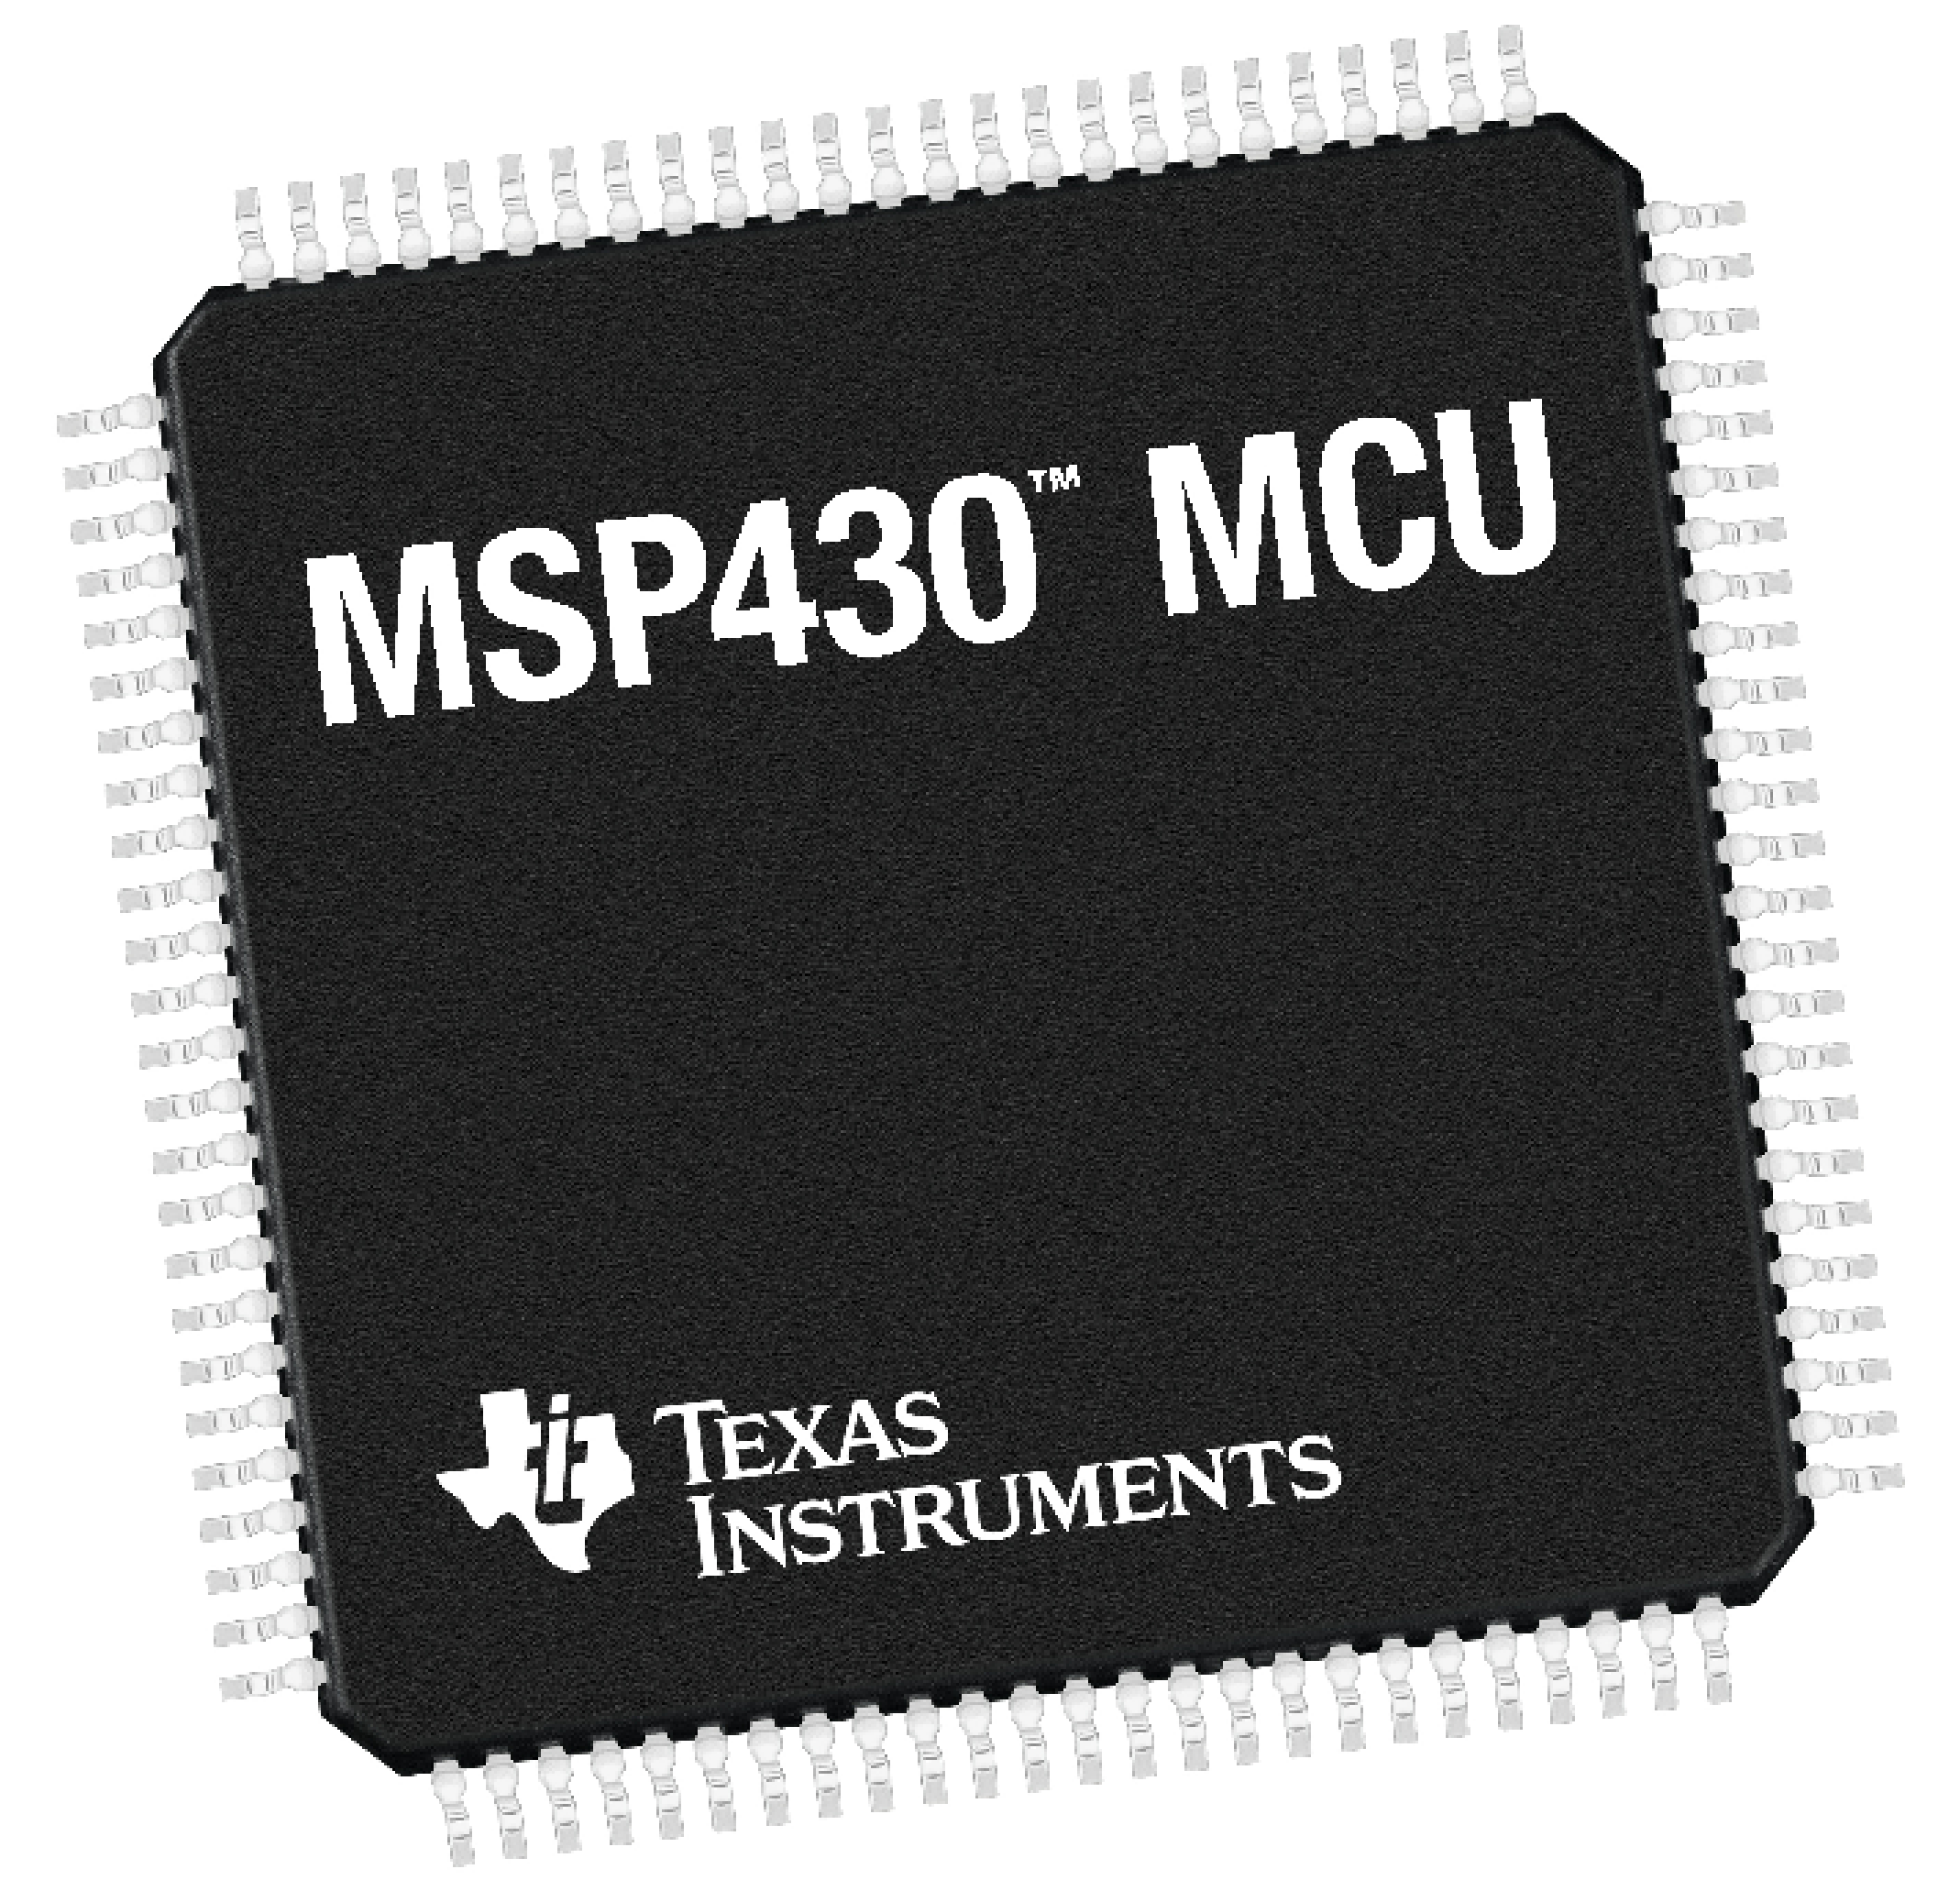
\includegraphics[scale=0.25]{images/msp430image}
\end{center}

\subsubsection{Background}
The MSP430\texttrademark is a line of ultra-low-power 16-bit microcontrollers produced by Texas Instruments. The microcontroller comes in several different flavors, which are outlined below.
\begin{center}
  \begin{tabular}{ l | l }
    Name & Features \\
    \hline
    1 Series & General purpose \\
    2 Series & General purpose (upgrade from the 1 Series) \\
    Value Line & Low cost \\
    4 Series with LCD & Integrated LCD controller \\
    5 Series & Integrated USB connectivity \\
    6 Series with LCD & Integrated USB connectivity and LCD controller \\
    FRAM Series & Includes FRAM (low-power, fast memory) \\
    Low Voltage Series & Low power \\
    RF SoC Series & Integrated RF tranceiver and LCD controller \\
    Fixed Function & Receives wireless power; pre-programmed \\
    Automotive & Certified by the Automotive Electronics Council \\
    Extended Temperature & Extended temperature range
  \end{tabular}
\end{center}
\mbox{}\\

\subsubsection{Hardware}
In order to be useful, a microcontroller development laboratory requires a method of programming, debugging, and testing the microcontrollers. In order to facilitate this, Texas Instruments has several off-the-shelf development board solutions for their MSP430\texttrademark line of microcontrollers. Since the MSP430\texttrademark microcontrollers do not all have the same number of pins, multiple development boards are needed to accommodate.
\begin{center}
  \begin{tabular}{ l | l }
    Name & Price \\
    \hline % XXX: Find solution for 8, 40, 24, 20 pin controllers
    MSP-TS430PW14 - MSP430 14-Pin Target Board & \$75.00 \\
    MSP-TS430PW28 - MSP430 28-Pin Socket Target Board & \$75.00 \\
    MSP-TS430DA38 - MSP430 38-Pin Target Board & \$75.00 \\
    MSP-TS430DL48 - MSP430 48-Pin Socket Target Board & \$75.00 \\
    MSP-TS430PM64 - MSP430 64-Pin Target Board & \$75.00 \\
    MSP-TS430PN80 - MSP430 80-Pin Target Board & \$75.00 \\
    MSP-TS430PZ100 - MSP430 100-Pin Target Board & \$75.00 \\
    MSP-TS430PZ100A - MSP430 100-Pin Target Board & \$75.00
  \end{tabular}
\end{center}
The Texas Instruments development boards also require a special flash emulation tool to program the device. This device is called the MSP-FET430UIF and in addition to providing programming capabilities, it also enables some debugging capabilities through the JTAG interface of the development boards. The cost of one MSP-FET430UIF is \$99.00. The MSP-FET430UIF is pictured below. \\ % XXX: Create figure and use reference to it
\begin{center}
  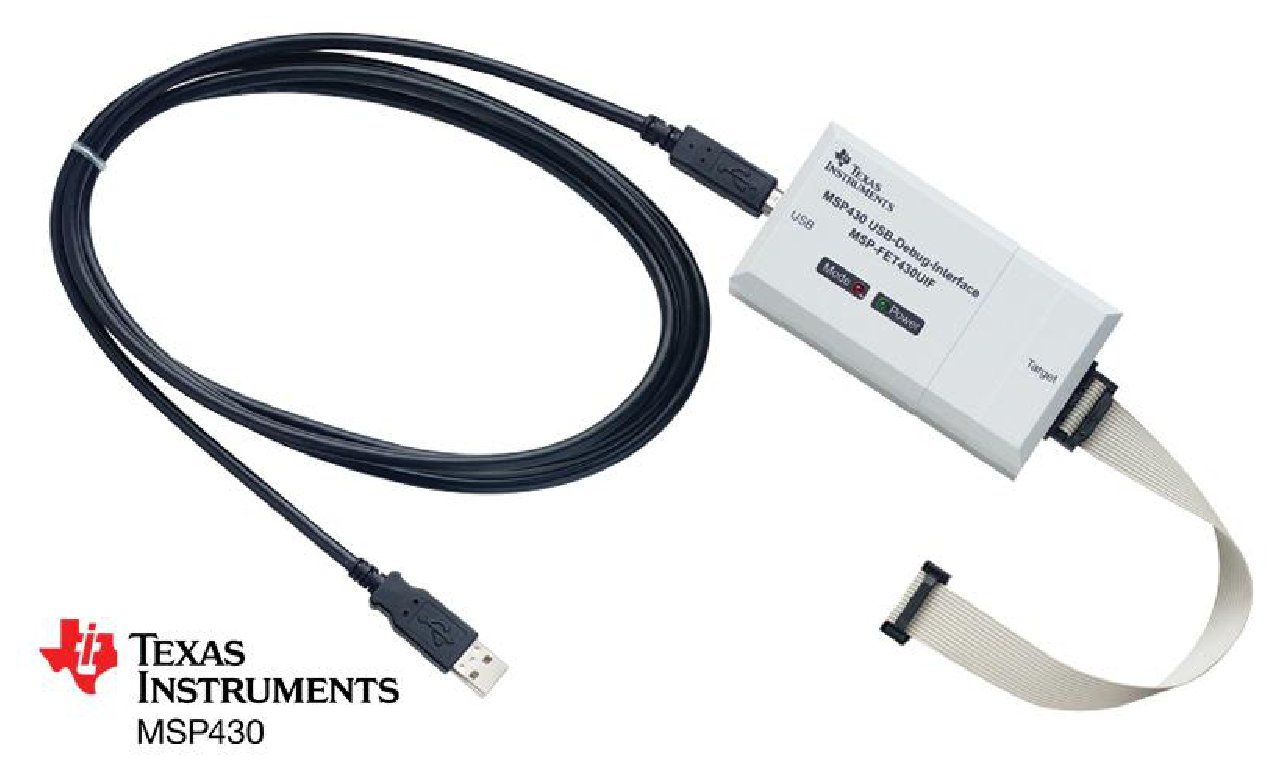
\includegraphics[scale=0.5]{images/fet430uif}
\end{center}
\mbox{}\\

\subsubsection{Software}
By their nature, embedded systems typically require user-defined code to be run on a microcontroller. In order to compile this user-defined code, program the microcontroller, and debug the system, software is required. Texas Instruments has a software package, Code Composer Studio\texttrademark, that performs all of these functions. It includes: 
\begin{itemize}
  \item Grace\texttrademark, a visual program to generate C code for interacting with peripherals
  \item SYS/BIOS, a real-time operating system for Texas Instruments microcontrollers
  \item A compiler tuned for the space limitations and performance characteristics of the MSP430
  \item Various system analysis and debugging tools
\end{itemize}
The above list is only a sample of some of the features of Code Composer Studio. The cost of this software package is \$795.00 for one floating license. The floating license allows for Code Composer Studio\texttrademark to be installed on multiple computers, but for only one user to use the application at any given time.

\subsection{Pico M-505 FPGA Module}
\begin{figure}[h!]
  \centering
  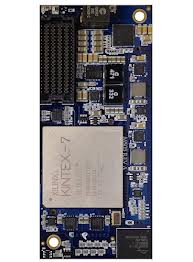
\includegraphics[scale=.5]{images/pico}
  \label{img:pico}
  \caption{Pico}
\end{figure}

\subsubsection{Description}
FPGA module utilizing a Xilinx Kintex-7 K410T, the world’s first 28nm
programmable logic device. Reasonably we can get twelve 505 modules and fully
set up two ex-500 backplanes.

\begin{figure}[h!]
  \centering
  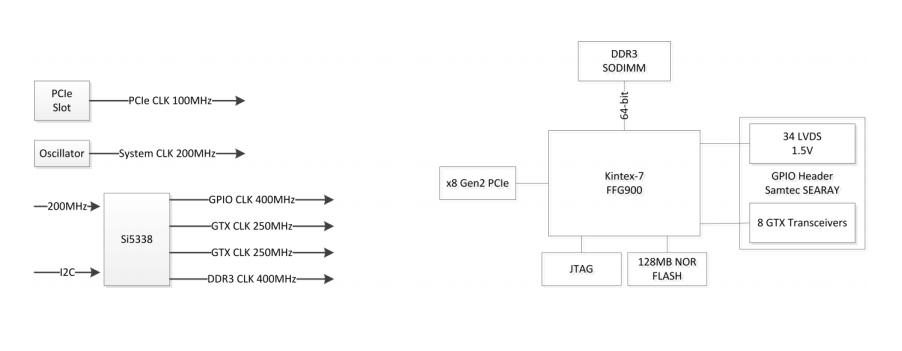
\includegraphics[scale=.5]{images/picoFlowChart.png}
  \label{img:picoFlow}
  \caption{Pico diagram}
\end{figure}

\subsubsection{Cost}

Not cheap, couldn't find any info online, will call Pico for more info.

\subsubsection{Why we need it}

Our lab needs a high performance FPGA setup for cryptography and bioinformatic projects

\subsubsection{Sensors}

None at the moment since we would be using our FPGA cluster for raw computing power

\subsubsection{Software}

Provided by Pico Computing with purchase.

\subsubsection{Additional Info}

Given a large enough budget, we could add a SC-5 SuperCluster with 48 Xilinx Kinetx-7's.

\begin{figure}[h!]
  \centering
  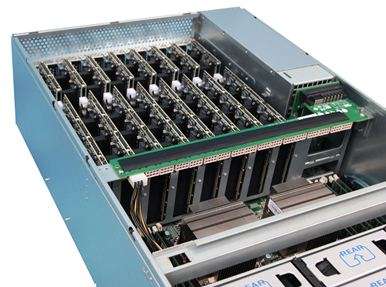
\includegraphics[scale=.5]{images/superCluster}
  \label{img:pico}
  \caption{SC-5 SuperCluster}
\end{figure}

\subsection{Papilio Pro FPGA Board}

\subsubsection{Description}
Essentially a cheap FPGA for hobbyists, the papilio has lots of add-
ons “aka wings” that make prototyping simple projects super easy. More of a
beginner/learning tool, it’s still pretty neat. Uses the Xilinx Spartan 3E FPGA

\begin{figure}[h!]
  \centering
  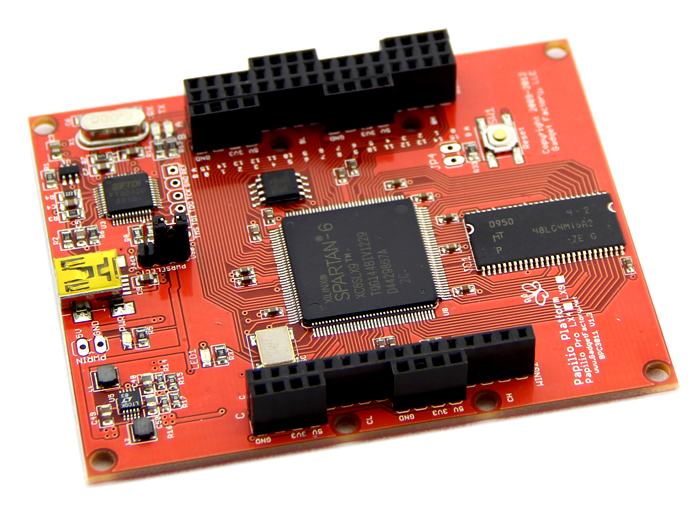
\includegraphics[scale=.5]{images/papilio}
  \label{img:pico}
  \caption{SC-5 SuperCluster}
\end{figure}


\subsection{PIC18 Series}
There are quite a few of the PIC18 devices, and any would really do for a learning setting
and are all relatively inexpensive and flexible for a variety of tasks be it communication, ADC,
or integration. All of the pic18f have internal oscillators so there wouldn't be a need for external
crystals or anything else of the sort that would cut down on the total cost of development. We
think that from a learning perspective, doing all of the work on a breadboard is essential to really
understanding how every pin of the PIC18. So, we dont believe a development kit would be very
necessary, however depending on the size and/or quality of lab we are looking at, may be a decent
option, so we will also discuss them.

\subsubsection{PIC18LF4550-I/P}

The PIC we would choose for a setting such as a university would be the
PIC18LF4550-I/P

\begin{figure}[h!]
  \centering
  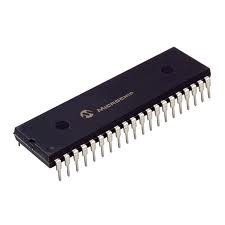
\includegraphics[scale=.5]{images/pic}
  \caption{PIC18LF4550-I/P}
  \label{img:pic}
\end{figure}


The pic18lf4550-I/P is an 8-bit microcontroller with three serial ports for usb, I2C, and SPI
communication. It can also be easily programmed for USART/UART communication it has 2048
bytes of ram and a CPU speed of 12 MIPS (so 48MHz). The memory type of this microcontroller
is flash, and has an available 32 KB to be programmed. It has a total of 40 pins, and is easily
worked into a breadboard for development because of its large pins.
Some of the neat features on this particular pic are its power saving modes, on-the-fly- mode
switching, multiple idle modes (can disable core of CPU and allow peripherals to continue to reduce
power consumption to about 4% of normal operations) .
It has four crystal modes, four external clock modes, and two internal clocks, so timing
considerations should really never be an issue for learning/development.
Also, new to the pic18 series is full USB communications (only up to usb 2.0 however).

\subsubsection{Why do we need it?}

The pic series of microcontrollers, from my perspective are used very frequently in industry and it
would be a good idea for students to get experience with this particular microcontroller architecture
so they are more prepared for work in a professional setting. The PIC microcontrollers are easyto learn, have great additional software and compilers, and a large support network. Due to being
manufactured my microchip, there is a high probability of receiving a quality product, with a
technical support back-up for any problems that may arise.
The PIC18LF4550 is very versatile and could be used for a lot of tasks, which we think is important
for a school setting as it could allow the biggest “bang-for-the-buck”, given that it can be used and
re-used for many different projects. The PIC18LF4550 would be a good fit for our lab because it
is also low cost and has quite a bit of free development tools which would help cut costs for our lab
as a whole. Seeing as, honestly, all one needs to start programming the pic microcontrollers is the
PIC18LF4550, a breadboard, and a programmer (as well as some free software).
Overall, the PIC18LF4550 is a cheap, easy to learn, useful, and supported microcontroller which
would be beneficial for students to learn before they graduate from school.
\subsubsection{Extra components}
As we said before, there are really no need for extra components when programming with the
pic18lf4550 as long as one has a pic, and a programmer.
So first up is the programmer:
The programmerthat we think would be best for the PIC18LF4550 is the PICKit2.
The PICkit2 is also developed by microchip, so compatibility is guaranteed. It is a cheap, fast, and
useful programmer with a couple of nice features.

\begin{enumerate}
\item It is an in-circuit debugger, so it works well with a breadboard. Just plug it into your circuit,
connect the power and programming pins to the PIC18LF4550.
\item It has an “on-the-fly” programming method that allows the pickit to reprogram a device with the
press of a single button.
\item The PICKit2 is open., meaning that its hardware and firmware are open to the public and as such,
has the availability to be used on linux machines.
\item Local UART tool (no need to use a hyperterminal to test uart)
When the PICKit2 is ordered it comes with driver software, an adapting usb cable, and Mplab IDE
software(also available free online).
\end{enumerate}

\begin{figure}[h]
  \centering
  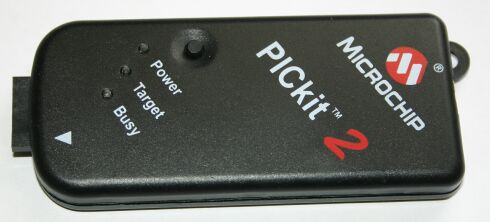
\includegraphics[scale=.5]{images/pickit}
-  \caption{Pickit 2}
  \label{img:pic}
\end{figure}

\subsubsection{Cost}
Thankfully, the microcontrollers and the programming/debugging hardware run very inexpensive,
The cost per MC is \hfill \\

\begin{tabular}{ l | l }
  Unit Quantity & Price \\
  \hline
  1-25 & 4.47 \\
  26-99 & 4.36 \\
  100+ & 4.26 \\
\end{tabular} 

\begin{tabular}{l | l}
  Unit Quantity & Price \\
  \hline
  1000-4999 & 3.92 \\
  5000+ & 3.72 \\
\end{tabular}
\hfill \\\\

\noindent
The cost for the pickit2 programmer/debugger with usb cable and software is 34.99 per unit.
As we am not entirely sure the scope of the lab and the number of lab machines to be equipped with
their own pickit2 (although they are very small and compact and could be moved from machine
to machine, and the software is free) we do not know how to add up the total costs for everything
involved.
However, as a rough estimate of three pickit2's in the lab, and a base order of 100 PIC18LF4550,
the total would come to 460.99 for a complete lab set up.

\subsubsection{Software Needed}
As stated before, if we do infact decide upon the pickit2, the software is already available in the
package in the form of microchip's MPLab.
This software is simply an IDE based off of netbeans(so also works great on linux) that allows the
user to write code, simulate that code, and add breakpoints.

\subsubsection{Other considerations}
There are a few other things that must be addressed for these pic microcontrollers. The compilers
used to program the PIC18LF4550 vary from company to company, or student to student. There a
a few free compilers such as MikroC, but we feel that sticking with Microchip's free compiler XC16
would be a good choice, just to keep consistent with the company that most of my suggested parts
are coming from. The XC compilers that microchip offers for free for download off of their website
are not as fully featured as their paid C30 compiler, or offer as much code optimization, but as I
said, is free. So, we suggest we use the XC16 compiler on any lab machine that would be used to
program PIC microcontrollers.
There are many additional things that would be useful for developing with pic18lf4550 such as
rs232 cables, USB cables, LED's, motors, and other such devices, but we did not include those
in the above description because they are really add-ons for projects that can be done with the
pic18lf4550.
I am assuming here that every student that were to use these machines would have their
own breadboards ( as are standard issue at michigan tech) . But for the prototyping of any
microcontroller or circuit, oscilloscopes are EXTREMELY useful. We know we have not yet
discussed oscilloscopes yet or if they will be a part of the lab, but maybe that is something to
discuss at a later date.


\section{Todo}
\begin{itemize}
\item Generate list of supported microcontrollers
\item Generate gantt chart for project timeline
\item For each microcontroller determine:
  \begin{itemize}
  \item Cost
  \item Necessary Software
  \item Necessary Adapters and Plugs
  \item Necessary equipment (shields/modules/dongles...)
  \end{itemize}
\item Design lab bench for fabrication of custom embedded devices
\end{itemize}

\end{document}
